\chapter{UCN Production and Detection}

The first UCN at TRIUMF (Nov.~2017) were produced by using the
vertical UCN source described in Sec.~\ref{vertical_source}. The
spallation neutrons were converted to UCN through phonon excitation in
the isotopically pure superfluid helium.  During data taking several
measurements were performed for better understandting of the vertical
UCN source and to help design the next generation UCN source. In this chapter,
the experiments are described and the result are shown.

Fig.~\ref{fig:volume_schematic} is a simple schematic of the UCN
production and detection volume.  Here volume $V_1$ is the production
volume before the valve where $N_1$ number of UCN is produced, $V_2$
is the secondary volume where $N_2$ number of UCN enters after opening
the valve , and $V_3$ is the detector volume with $N_3$ number of UCN.



\begin{figure}[h]
  \centering
  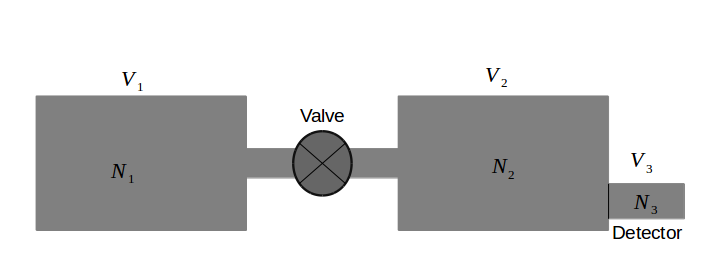
\includegraphics[width=0.9\textwidth]{volume_schematic.png}
  \caption{Schematic drawing of a UCN source. $V_1$ is the production
    volume with $N_1$ number of UCN, $V_2$ is the secondary volume
    where $N_2$ number of UCN exist and $V_3$ is the detector with
    $N_3$ number of UCN. }
  \label{fig:volume_schematic}
\end{figure}


When the beam is on and the valve is closed, the number of UCN in
$V_1$ goes up while the total number of UCN in $V_2$ and $V_3$ is
zero. This is described as 

\begin{equation}
  \label{eqn:dndt}
\frac{dN_1}{dt} = P - \frac{N_1}{\tau_1}  
\end{equation}
where $P$ is the UCN production rate in the source as describe in
Sec.~\ref{sec:UCN_production} and $\tau_1$ is the UCN storage lifetime
in the source.

After the beam is turned off, the valve is opened and the UCN travels
to the volume $V_2$ and eventually $V_3$. The valve is usually left
open for 2 to 3 minutes. The UCN trade between $V_1$, $V_2$ and $V_3$
is described by the differential Eqn.~\ref{eqn:alldndt}.

\begin{equation}
  \label{eqn:alldndt}
  \begin{aligned}
    \frac{dN_1}{dt} =&- \frac{N_1}{\tau_{c,1}} - \frac{N_1}{\tau_1} + \frac{N_2}{\tau_{c,2}}  \\
    \frac{dN_2}{dt} =& \frac{N_1}{\tau_{c,1}} - \frac{N_2}{\tau_{c,2}} - \frac{N_2}{\tau_2} - \frac{N_2}{\tau_{c,3}} \\
    \frac{dN_3}{dt} =& \frac{N_2}{\tau_{c,3}}.
  \end{aligned}
\end{equation}


In these equations, \large $\frac{dN_1}{dt}$ \normalsize shows the
change in the UCN counts over time in $V_1$,~\large $\frac{dN_2}{dt}$
\normalsize shows the change in the UCN counts in $V_2$ and \large
$\frac{dN_3}{dt}$ \normalsize is change in the UCN count in $V_3$
which is the detector all after the valve is opened.

The total number of UCN in $V_1$ depends on three things. The UCN that
get into $V_2$~\large($\frac{N_1}{\tau_{c,1}}$) \normalsize, the UCN that is lost
with the storage lifetime of $\tau_1$, and the UCN that bounce back from
$V_2$ to $V_1$~\large ($\frac{N_2}{\tau_{c,2}}$) \normalsize.

In $V_2$, some UCN cross from $V_1$ to $V_2$~ \large
($\frac{N_1}{\tau_{c,1}}$) \normalsize, some get lost with the
lifetime of $\tau_2$~\large ($\frac{N_2}{\tau_2}$) \normalsize, some
cross the gate valve to go back to $V_1$~ \large
($\frac{N_2}{\tau_{c,2}}$)\normalsize and some get to the detector
~\large ($\frac{N_2}{\tau_{c,3}}$) \normalsize. The rate of the UCN
detection $\frac{dN_3}{dt}$ is the number of UCN crossing from $V_2$.
The end of the measurement cycle is determined by the valve closing
time.

Solving these equation could give an estimate of how many UCN exist in
each volume. The process described above is refered to the UCN
production in {\it {batch mode}}. The UCN rate for 1~$\mu$A beam current
and 60~s irradiation time is shown in Fig.~\ref{fig:UCNRate}.


\begin{figure}[h]
  \centering
  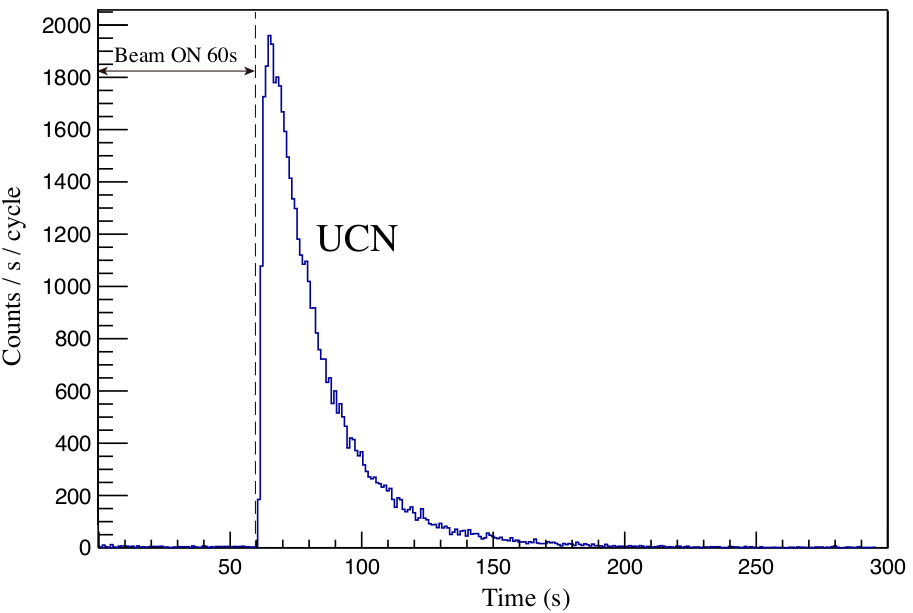
\includegraphics[width=0.7\textwidth]{UCNRate.png}
  \caption{The figure shows the UCN rate at 60~s irradiation time and
    1~$\mu$A beam current. In this case, the UCN gate valve is opened
    immediately after the end of irradiation. At this time, the UCN
    rate reaches the peak of about 2000 UCN/s. The UCN rate decays
    down to zero. The Valve is left open for 120~s. }
  \label{fig:UCNRate}
\end{figure}



A 3D drawing of the experimental setup is shown in
Fig.~\ref{fig:Source_all}. In this case, $V_1$ is the UCN source
bottle and the horizontal section of the UCN guide before the UCN gate
valve and $V_2$ and $V_3$ are the volumes after the UCN valve and the
detector volume respectively.




Another possible mode of operation is when we leave the UCN valve open
while irradiating the target. This is called the {\it{ steady-state}}
mode where we have a constant stream of UCN to the main detector.


\begin{figure}[h]
  \centering
  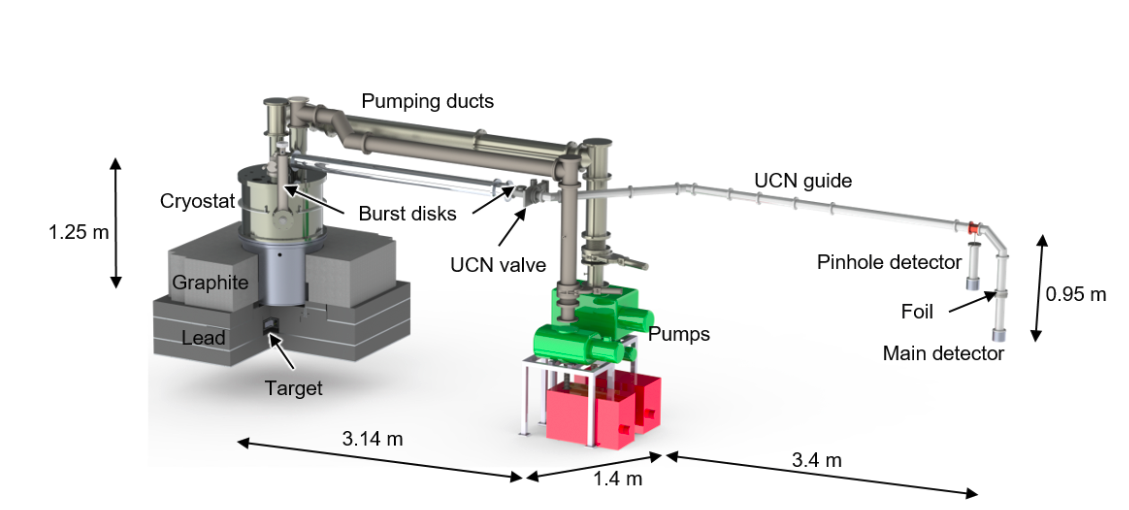
\includegraphics[width=1.1\textwidth]{Source_all.png}
  \caption{The UCN source and the guide geometry at TRIUMF }
  \label{fig:Source_all}
\end{figure}


The following sections are focused on the result of the UCN yield
optimization, the UCN storage lifetime measurements, the two detector
comparisons and the UCN guide transmission measurements.




\section{UCN Count Measurement \label{UCNCounts}}

The total number of produced UCN in the vertical source, $N$,
at a certain time t$_i$ is the integration of eqn.~\ref{eqn:dndt}
\begin{equation}
  \label{eq:totalUCN}
  N = P \tau_1\left[ 1- \exp \left(\frac{t_i }{ \tau_1}\right) \right]
\end{equation}
where the UCN storage lifetime $\tau_1$ is given by

\begin{equation}
  \label{eqn:tau1}
  \frac{1}{\tau_1} = \frac{ f_\mathrm{He,1}}{\tau_\mathrm{He}} + \frac{1}{\tau_\mathrm{wall,1}}.
\end{equation}

The storage lifetime consists of two terms: the upscattering rate in
the superfluid helium and the loss rate in the UCN guide walls. The
volume in which these UCN are produced consists of the UCN bottle as
well as the horizontal guide section before the gate valve~(See
Fig.~\ref{fig:Source_all}).This volume is not fully filled with the
superfluid helium. As a result, $ f_\mathrm{He,1}$ is the probablity
of UCN being in the superfluid helium and \large
$\frac{ f_\mathrm{He,1}}{\tau_\mathrm{He}}$ \normalsize is the
upscattering rate in the superfluid helium which is a function of the
superfluid helium temperature~(See Sec.~\ref{sec:upscattering}. The
loss rate in the guide walls is $\frac{1}{\tau_\mathrm{wall,1}}$.

After the valve is opened, the total UCN lifetime is

\begin{equation}
  \label{eqn:tau2}
  \frac{1}{\tau_2} = \frac{ f_\mathrm{He,2}}{\tau_\mathrm{He}} + \frac{1}{\tau_\mathrm{wall,2}}+\frac{1}{\tau_d}
\end{equation}
where $\tau_d^{-1}$ is the loss rate in the detector.

plans for tomorrow thursday:
1. Make a graph with vertical  lines to show when the valve is opened nad when is closed.
2. finish this section of counts.
3. start the storage lifetime section.

\section{Storage Lifetime Measurements}

\section{Heater Tests of The Source}

\section{Detector Comparison}
Using the rotary valve

\section{Background Measurements}
With Ni foil

\section{UCN guide Transmission Measurements}

\section{Result And Conclusion}

%\begin{description}
%\item{I think this belongs to this chapter: UCN production by
%  multiphonon excitation in superfluid helium (I can use my candidacy
%  report for this part as a start)}
  
%\item{Some information about the detector}
  
%\item{UCN data goes here}
  
%\item{what else?}
%\end{description}
